\subsection{Messverfahren}
\paragraph{Aufgabe 1:} Skizze des Versuchsaufbaus im Messprotokoll.

\paragraph{Aufgabe 2:} Inbetriebnahme des GM-ZR: Mithilfe der akustischen Ausgabe der Zerfallsdetektion wird die Einsatzspannung \(U_0\)(schlagartiges Auftauchen des akustischen Signals) bestimmt und anschließend bei einer Torzeit von \(t=\qty{30}{\s}\) und schrittweiser Spannungserhöhung die Ereigniszahl \(N\) bestimmt. 

\paragraph{Aufgabe 3:} Plateauanstieg: Das Präparat wird so nahe wie möglich an das Zählrohr gestellt und für \(U_0\) sowie \(U_0+\qty{100}{\volt}\) für \(\qtylist{60;180}{\s}\) die Ereigniszahl gemessen. 

\paragraph{Aufgabe 4\&5:} 2000,5000 Messungen der Zerfallszahl pro \(t=\qtylist{0.5;0.1}{\s}\), die in ein Histogramm aufgetragen werden. Bei der ersten Messung wurde die Zerfallsrate auf \(n=\qtyrange{150}{160}{\per\s}\), bei der zweiten auf \(n=\qtyrange{40}{50}{\per\s}\) eingestellt. Dies bewirkt einen geringen Mittelwert von gemessenen Ereignissen pro Zeit \(t\) bei der zweiten Verteilung. 
\vfill
\subsection{Messprotokoll}
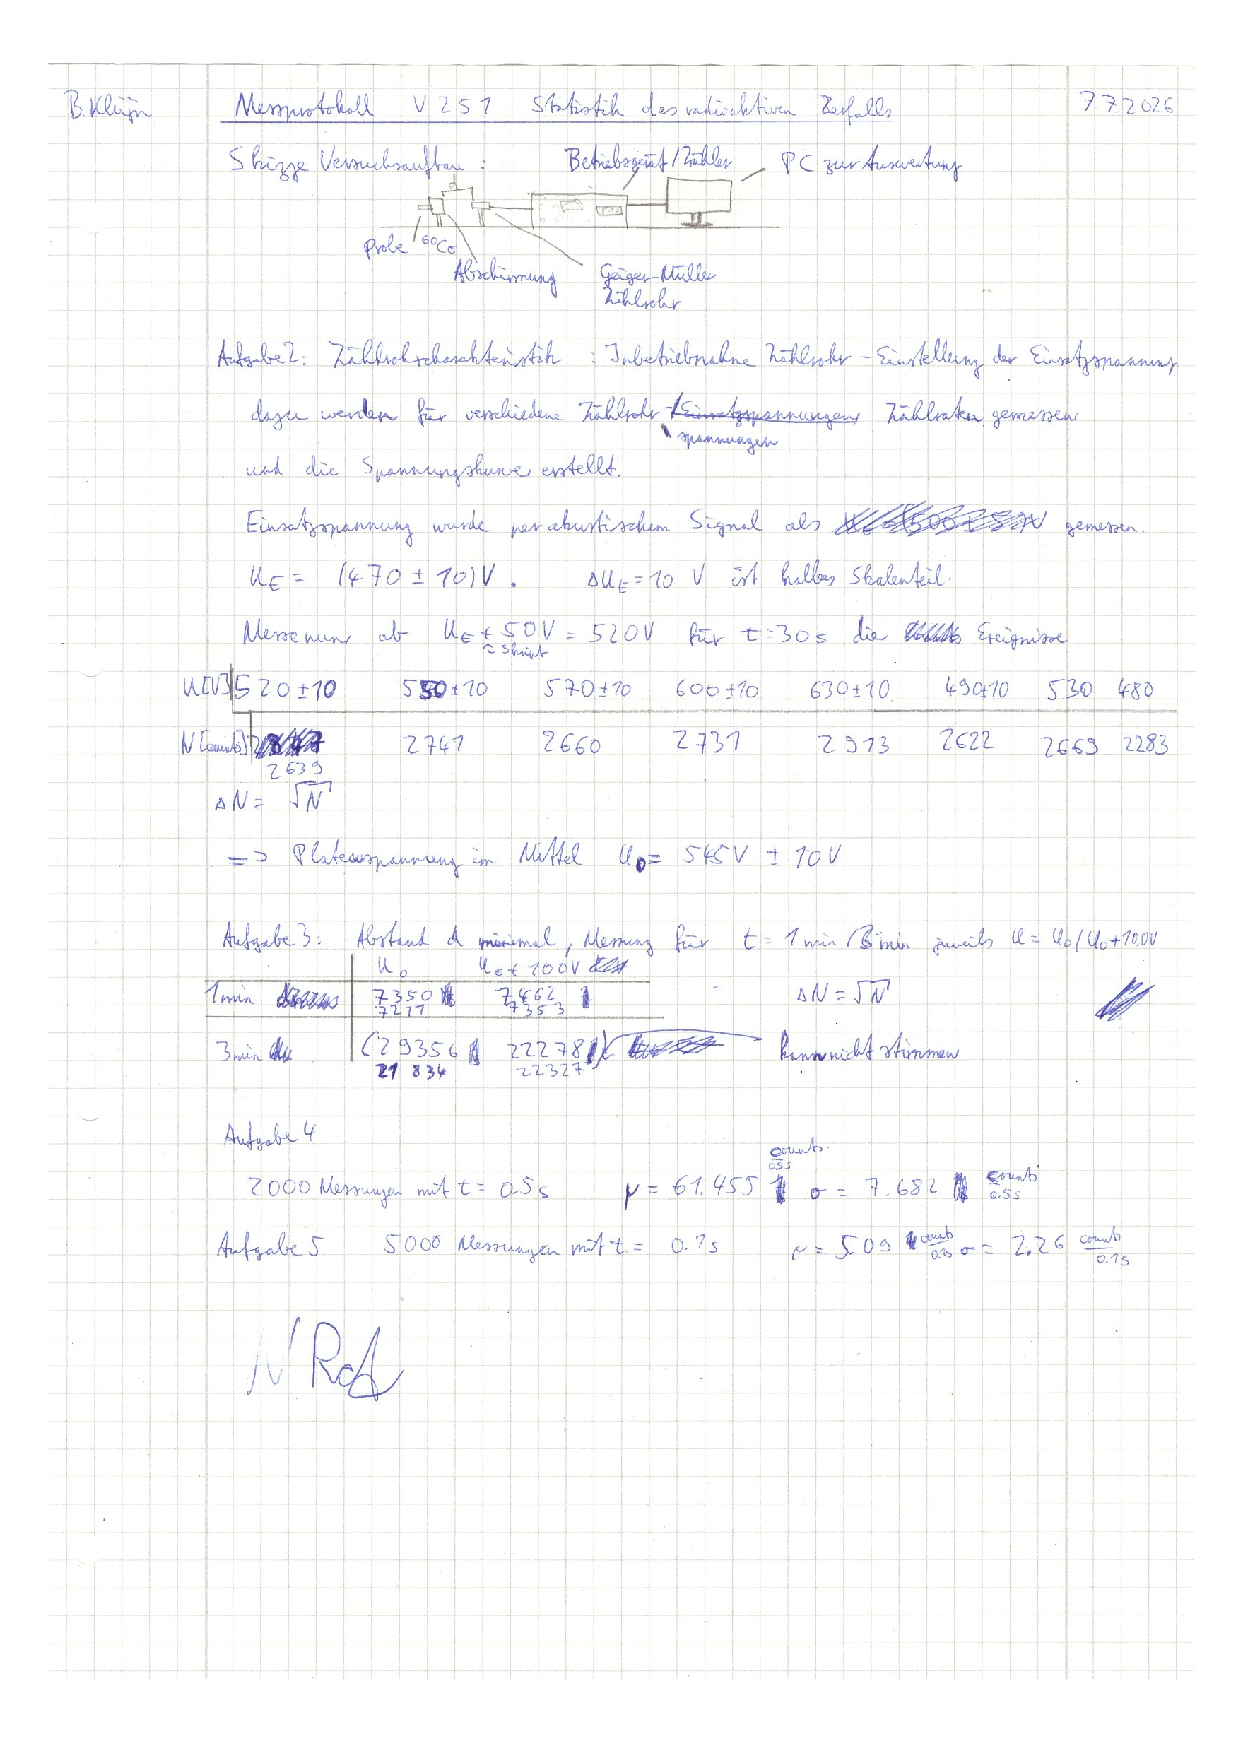
\includepdf[pages=-]{./images/251.pdf}
% heibox.uni-heidelberg.de/d/a48f9d7b91264990a16e/
